\begin{figure}
    \centering
    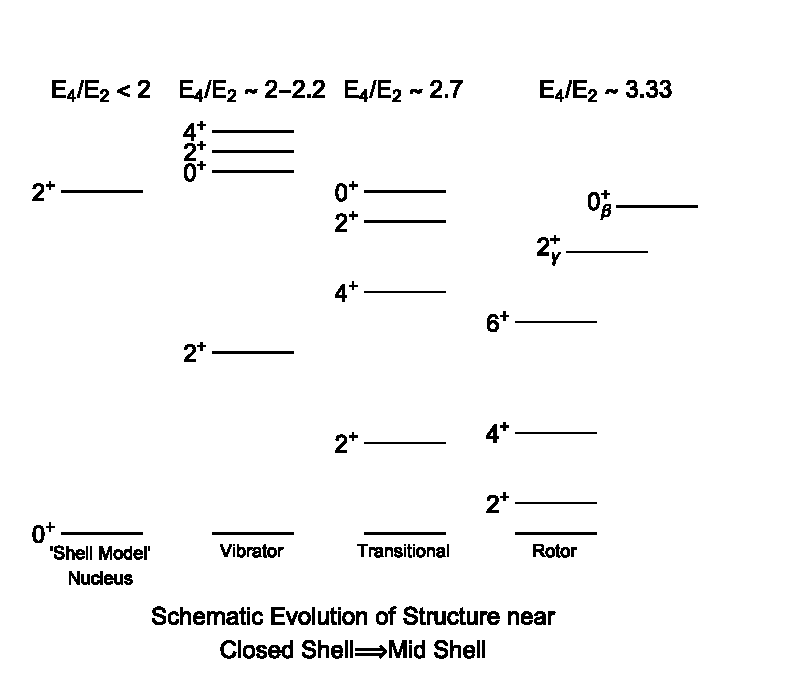
\includegraphics[scale=1]{Introduction_Figs/ShellStructureEvolution.eps}
    \caption{Cartoon of what excited states built upon different types of nuclei looks like. The closed shell has a large gap between the ground state and first excited state. In the vibrator model, this gap is lower, and a gap of comparable size exists before a cluster of states occurs. In the rotor model, the spacing follows a spacing pattern of $J_f(J_f+1)-J_i(J_i+1)$, with $\gamma$ and $\beta$ vibrations also coming into play. The trasitional area between vibrator and rotor shows a shift between the two, with the clustered states of the vibrator model beginning to space out.}
    \label{fig:statestructure}
\end{figure}